\documentclass[border=10pt]{standalone}
\usepackage{tikz}
\usetikzlibrary{arrows,positioning,shapes.geometric}
\begin{document}
\







\tikzset{every picture/.style={line width=0.75pt}} %set default line width to 0.75pt        

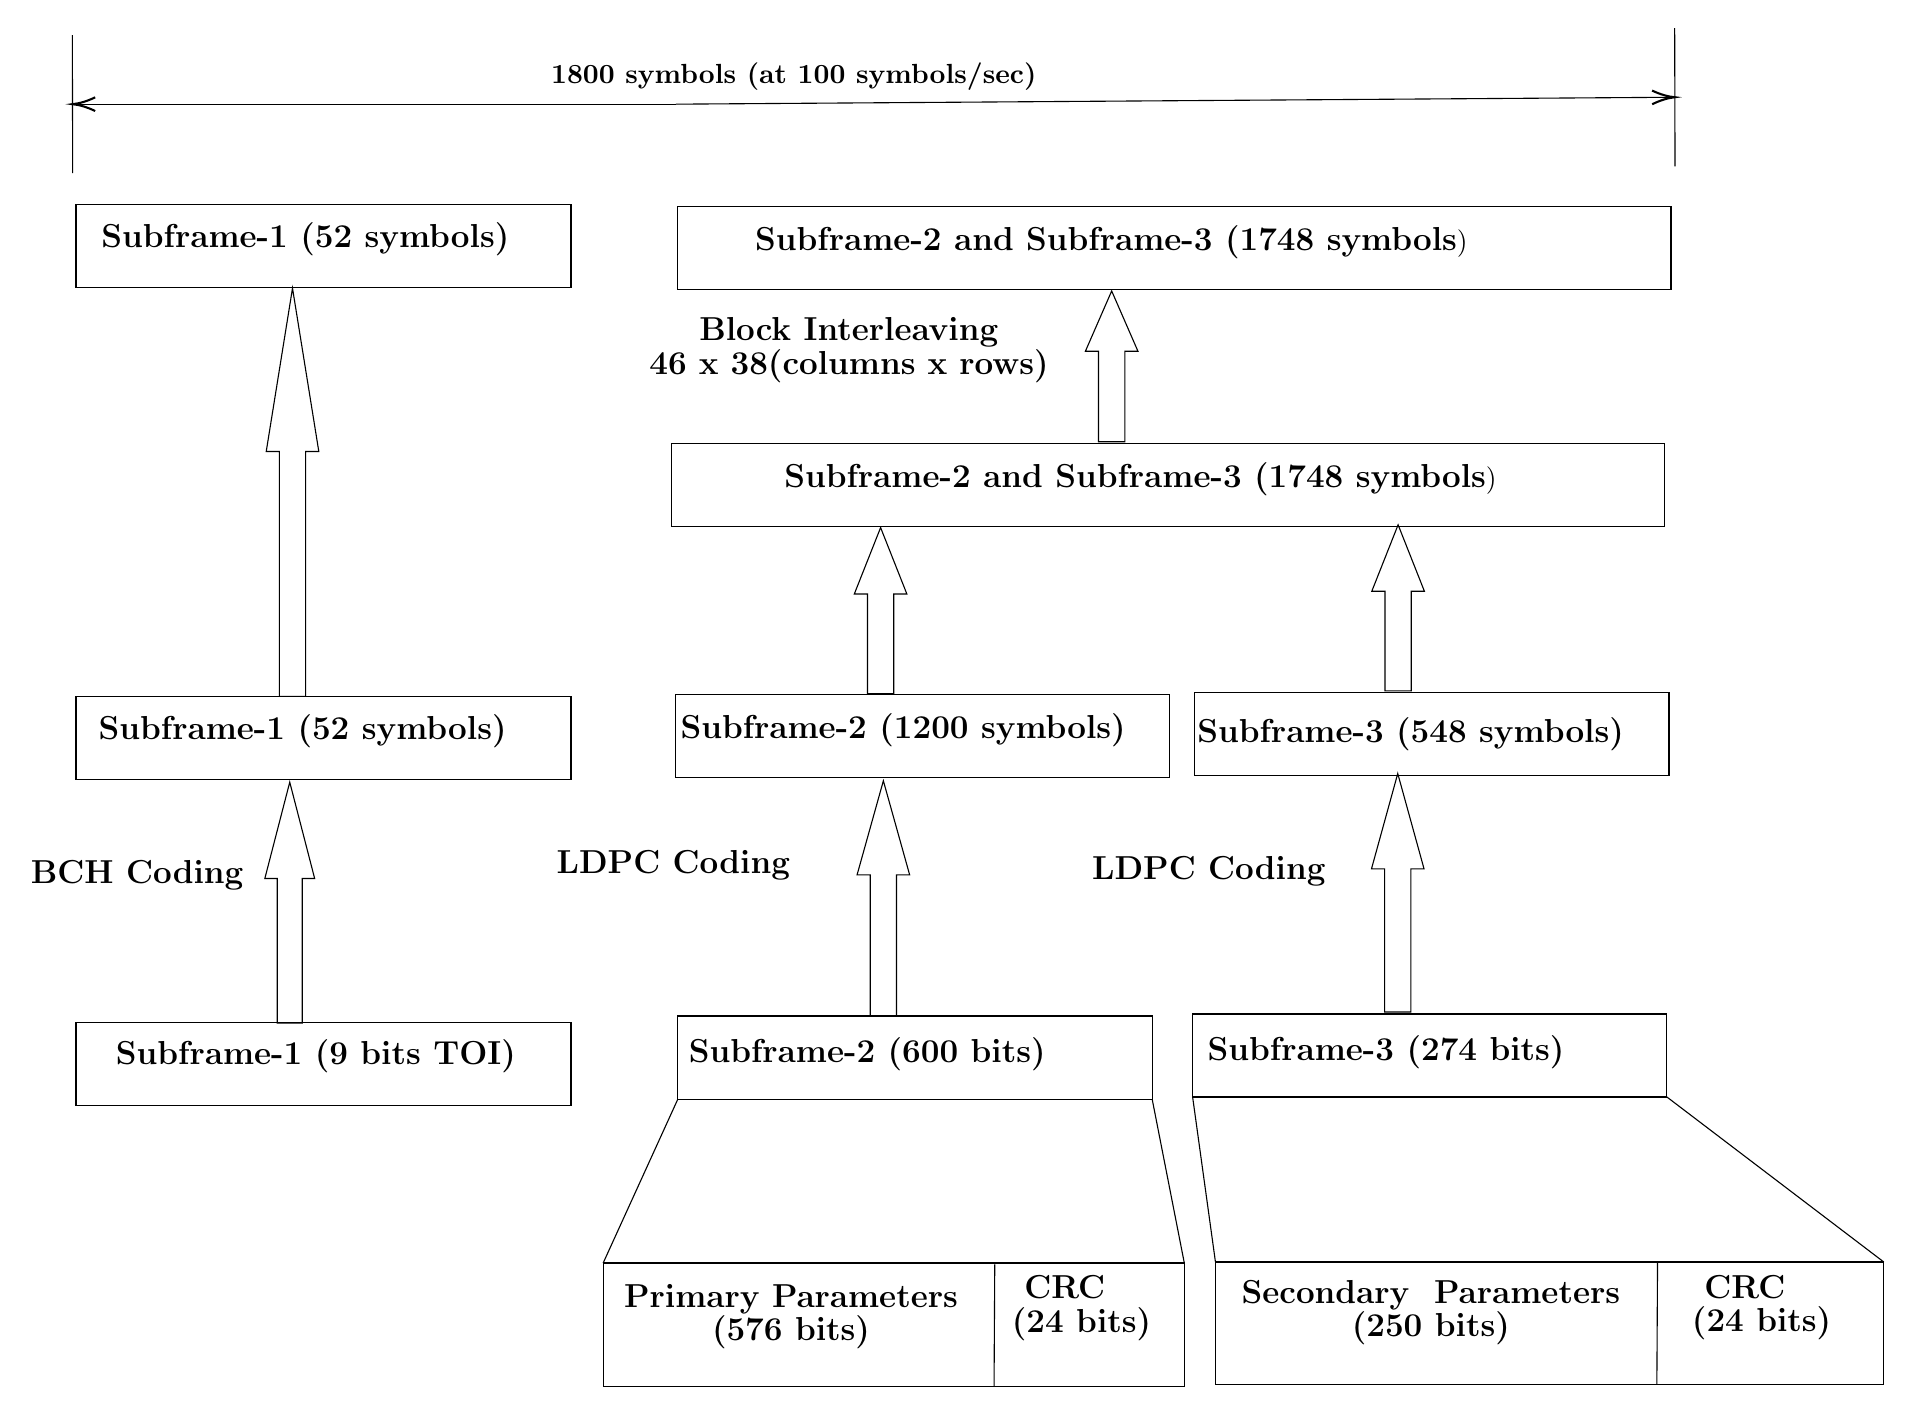
\begin{tikzpicture}[x=0.75pt,y=0.75pt,yscale=-1,xscale=1]
%uncomment if require: \path (0,975); %set diagram left start at 0, and has height of 975

%Shape: Rectangle [id:dp9370539777491956] 
\draw   (49,120) -- (287.5,120) -- (287.5,160) -- (49,160) -- cycle ;
%Shape: Rectangle [id:dp8458590125468772] 
\draw   (339,121) -- (817.5,121) -- (817.5,161) -- (339,161) -- cycle ;
%Shape: Rectangle [id:dp5265053229640352] 
\draw   (49,357) -- (287.5,357) -- (287.5,397) -- (49,397) -- cycle ;
%Shape: Rectangle [id:dp19373241489795656] 
\draw   (49,514) -- (287.5,514) -- (287.5,554) -- (49,554) -- cycle ;
%Shape: Rectangle [id:dp9214975483957203] 
\draw   (336,235) -- (814.5,235) -- (814.5,275) -- (336,275) -- cycle ;
%Shape: Rectangle [id:dp622727042927181] 
\draw   (338,356) -- (576,356) -- (576,396) -- (338,396) -- cycle ;
%Shape: Rectangle [id:dp8460025972970162] 
\draw   (588,355) -- (816.5,355) -- (816.5,395) -- (588,395) -- cycle ;
%Shape: Rectangle [id:dp7112505456045537] 
\draw   (339,511) -- (567.5,511) -- (567.5,551) -- (339,551) -- cycle ;
%Shape: Rectangle [id:dp10789004787398071] 
\draw   (587,510) -- (815.5,510) -- (815.5,550) -- (587,550) -- cycle ;
%Shape: Rectangle [id:dp9531343099401215] 
\draw   (303,630) -- (583,630) -- (583,689.5) -- (303,689.5) -- cycle ;
%Straight Lines [id:da2637886032876362] 
\draw    (491.67,630.67) -- (491.33,689.67) ;
%Shape: Rectangle [id:dp15054806924035746] 
\draw   (598,629.5) -- (920,629.5) -- (920,688.5) -- (598,688.5) -- cycle ;
%Straight Lines [id:da4849829306936325] 
\draw    (811,629.33) -- (810.67,688.33) ;
%Straight Lines [id:da806516666152795] 
\draw    (815.5,550) -- (920,629.5) ;
%Straight Lines [id:da9179451138258451] 
\draw    (587,550) -- (598,629.5) ;
%Straight Lines [id:da6946178367477058] 
\draw    (567.5,551) -- (583,630) ;
%Straight Lines [id:da7043991691304728] 
\draw    (339,551) -- (303,630) ;
%Up Arrow [id:dp7833254845115745] 
\draw   (140,444.73) -- (152,398.33) -- (164,444.73) -- (158,444.73) -- (158,514.33) -- (146,514.33) -- (146,444.73) -- cycle ;
%Up Arrow [id:dp8574230361325054] 
\draw   (140.67,239) -- (153.33,160.33) -- (166,239) -- (159.67,239) -- (159.67,357) -- (147,357) -- (147,239) -- cycle ;
%Up Arrow [id:dp47898198519742263] 
\draw   (535.33,190.73) -- (548,161.67) -- (560.67,190.73) -- (554.33,190.73) -- (554.33,234.33) -- (541.67,234.33) -- (541.67,190.73) -- cycle ;
%Up Arrow [id:dp05098847612391322] 
\draw   (424,307.67) -- (436.67,275.67) -- (449.33,307.67) -- (443,307.67) -- (443,355.67) -- (430.33,355.67) -- (430.33,307.67) -- cycle ;
%Up Arrow [id:dp650262231566618] 
\draw   (673.33,306.33) -- (686,274.33) -- (698.67,306.33) -- (692.33,306.33) -- (692.33,354.33) -- (679.67,354.33) -- (679.67,306.33) -- cycle ;
%Up Arrow [id:dp6627405157997192] 
\draw   (425.33,443) -- (438,397.67) -- (450.67,443) -- (444.33,443) -- (444.33,511) -- (431.67,511) -- (431.67,443) -- cycle ;
%Up Arrow [id:dp12275307707624372] 
\draw   (673.17,440.11) -- (685.83,394.17) -- (698.5,440.11) -- (692.17,440.11) -- (692.17,509.03) -- (679.5,509.03) -- (679.5,440.11) -- cycle ;
%Straight Lines [id:da5731387861346273] 
\draw    (338,71.67) -- (817.33,68.35) ;
\draw [shift={(819.33,68.33)}, rotate = 179.6] [color={rgb, 255:red, 0; green, 0; blue, 0 }  ][line width=0.75]    (10.93,-3.29) .. controls (6.95,-1.4) and (3.31,-0.3) .. (0,0) .. controls (3.31,0.3) and (6.95,1.4) .. (10.93,3.29)   ;
%Straight Lines [id:da5317419155557673] 
\draw    (338,71.67) -- (49.33,71.67) ;
\draw [shift={(47.33,71.67)}, rotate = 360] [color={rgb, 255:red, 0; green, 0; blue, 0 }  ][line width=0.75]    (10.93,-3.29) .. controls (6.95,-1.4) and (3.31,-0.3) .. (0,0) .. controls (3.31,0.3) and (6.95,1.4) .. (10.93,3.29)   ;
%Straight Lines [id:da36686612438372257] 
\draw    (47.25,38.42) -- (47.42,104.92) ;
%Straight Lines [id:da25579383874478734] 
\draw    (819.25,35.08) -- (819.42,101.58) ;

% Text Node
\draw (60,127.67) node [anchor=north west][inner sep=0.75pt]   [align=left] {\textbf{{\large Subframe-1 (52 symbols)}}};
% Text Node
\draw (375,129) node [anchor=north west][inner sep=0.75pt]   [align=left] {\textbf{{\large Subframe-2 and Subframe-3 (1748 symbols}})};
% Text Node
\draw (58.67,364.67) node [anchor=north west][inner sep=0.75pt]   [align=left] {\textbf{{\large Subframe-1 (52 symbols)}}};
% Text Node
\draw (67,521) node [anchor=north west][inner sep=0.75pt]   [align=left] {\textbf{{\large Subframe-1 (9 bits TOI)}}};
% Text Node
\draw (389,243) node [anchor=north west][inner sep=0.75pt]   [align=left] {\textbf{{\large Subframe-2 and Subframe-3 (1748 symbols}})};
% Text Node
\draw (339,364) node [anchor=north west][inner sep=0.75pt]   [align=left] {\textbf{{\large Subframe-2 (1200 symbols)}}};
% Text Node
\draw (588,366) node [anchor=north west][inner sep=0.75pt]   [align=left] {\textbf{{\large Subframe-3 (548 symbols)}}};
% Text Node
\draw (343,520) node [anchor=north west][inner sep=0.75pt]   [align=left] {\textbf{{\large Subframe-2 (600 bits)}}};
% Text Node
\draw (593,519) node [anchor=north west][inner sep=0.75pt]   [align=left] {\textbf{{\large Subframe-3 (274 bits)}}};
% Text Node
\draw (311,639) node [anchor=north west][inner sep=0.75pt]   [align=left] {\begin{minipage}[lt]{121.84pt}\setlength\topsep{0pt}
\begin{center}
\textbf{{\large Primary Parameters }}\\\textbf{{\large (576 bits)}}
\end{center}

\end{minipage}};
% Text Node
\draw (498.67,635) node [anchor=north west][inner sep=0.75pt]   [align=left] {\textbf{{\large  \ CRC }}\\\textbf{{\large (24 bits)}}};
% Text Node
\draw (605.67,637) node [anchor=north west][inner sep=0.75pt]   [align=left] {\begin{minipage}[lt]{142.26pt}\setlength\topsep{0pt}
\begin{center}
\textbf{{\large Secondary \ Parameters }}\\\textbf{{\large (250 bits)}}
\end{center}

\end{minipage}};
% Text Node
\draw (826.33,634.67) node [anchor=north west][inner sep=0.75pt]   [align=left] {\textbf{{\large  \ CRC }}\\\textbf{{\large (24 bits)}}};
% Text Node
\draw (276.67,50.33) node [anchor=north west][inner sep=0.75pt]   [align=left] {\textbf{1800 symbols (at 100 symbols/sec)}};
% Text Node
\draw (26,434.67) node [anchor=north west][inner sep=0.75pt]   [align=left] {\textbf{{\large BCH Coding}}};
% Text Node
\draw (279.33,430) node [anchor=north west][inner sep=0.75pt]   [align=left] {\textbf{{\large LDPC Coding}}};
% Text Node
\draw (537.33,432.67) node [anchor=north west][inner sep=0.75pt]   [align=left] {\textbf{{\large LDPC Coding}}};
% Text Node
\draw (324,173.33) node [anchor=north west][inner sep=0.75pt]   [align=left] {\begin{minipage}[lt]{144.27pt}\setlength\topsep{0pt}
\begin{center}
\textbf{{\large Block Interleaving}}\\\textbf{{\large 46 x 38(columns x rows)}}
\end{center}

\end{minipage}};


\end{tikzpicture}



   
\end{document}


